\chapter{Used data}

\section{Data science view on datasets}

With the dataset creation understood from the real-world side, let us now look at how it is handled from a machine-learning point of view. 

\subsection{Raw data intuition}

The raw input into any of our models is the protein's 3D structure. This is represented by a point cloud on the protein's surface. Each point has a feature vector attached, which represents the chemical properties of the given accessible surface patch. Each point also has an LBS class, which the model trains and predicts. These can be seen in the figure~\ref{fig:class_point_cloud}.

\begin{figure}
    \centering
    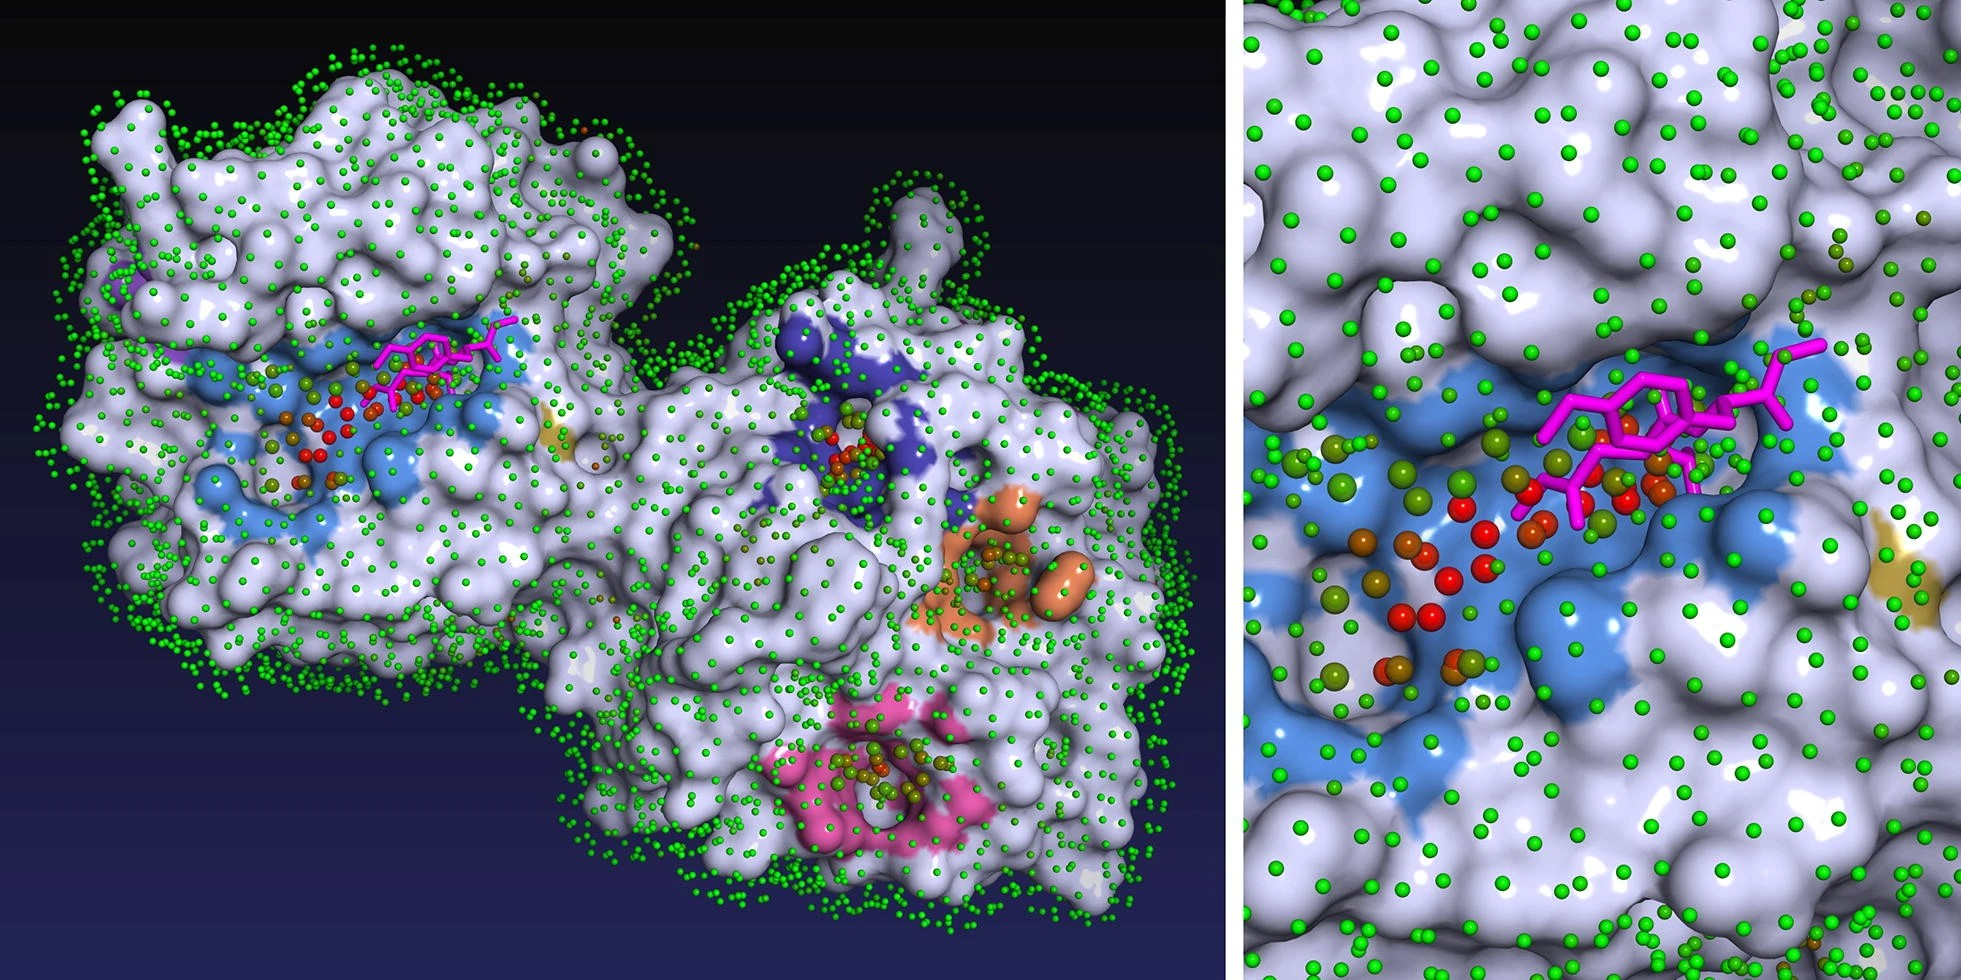
\includegraphics[width=1\linewidth]{p2rank.jpg}
    \caption{Visualization of a molecule taken directly from \cite{P2RANK}. The protein surface is covered by SAS points represented by green to red points representing predicted ligandability  (from 0 = green to 1 = red). The largest pocket (shown in the close-up) is indeed a correctly predicted true binding site that binds a known ligand (magenta). }
    \label{fig:p2rank_visualization}
\end{figure}

\begin{figure}
    \centering
    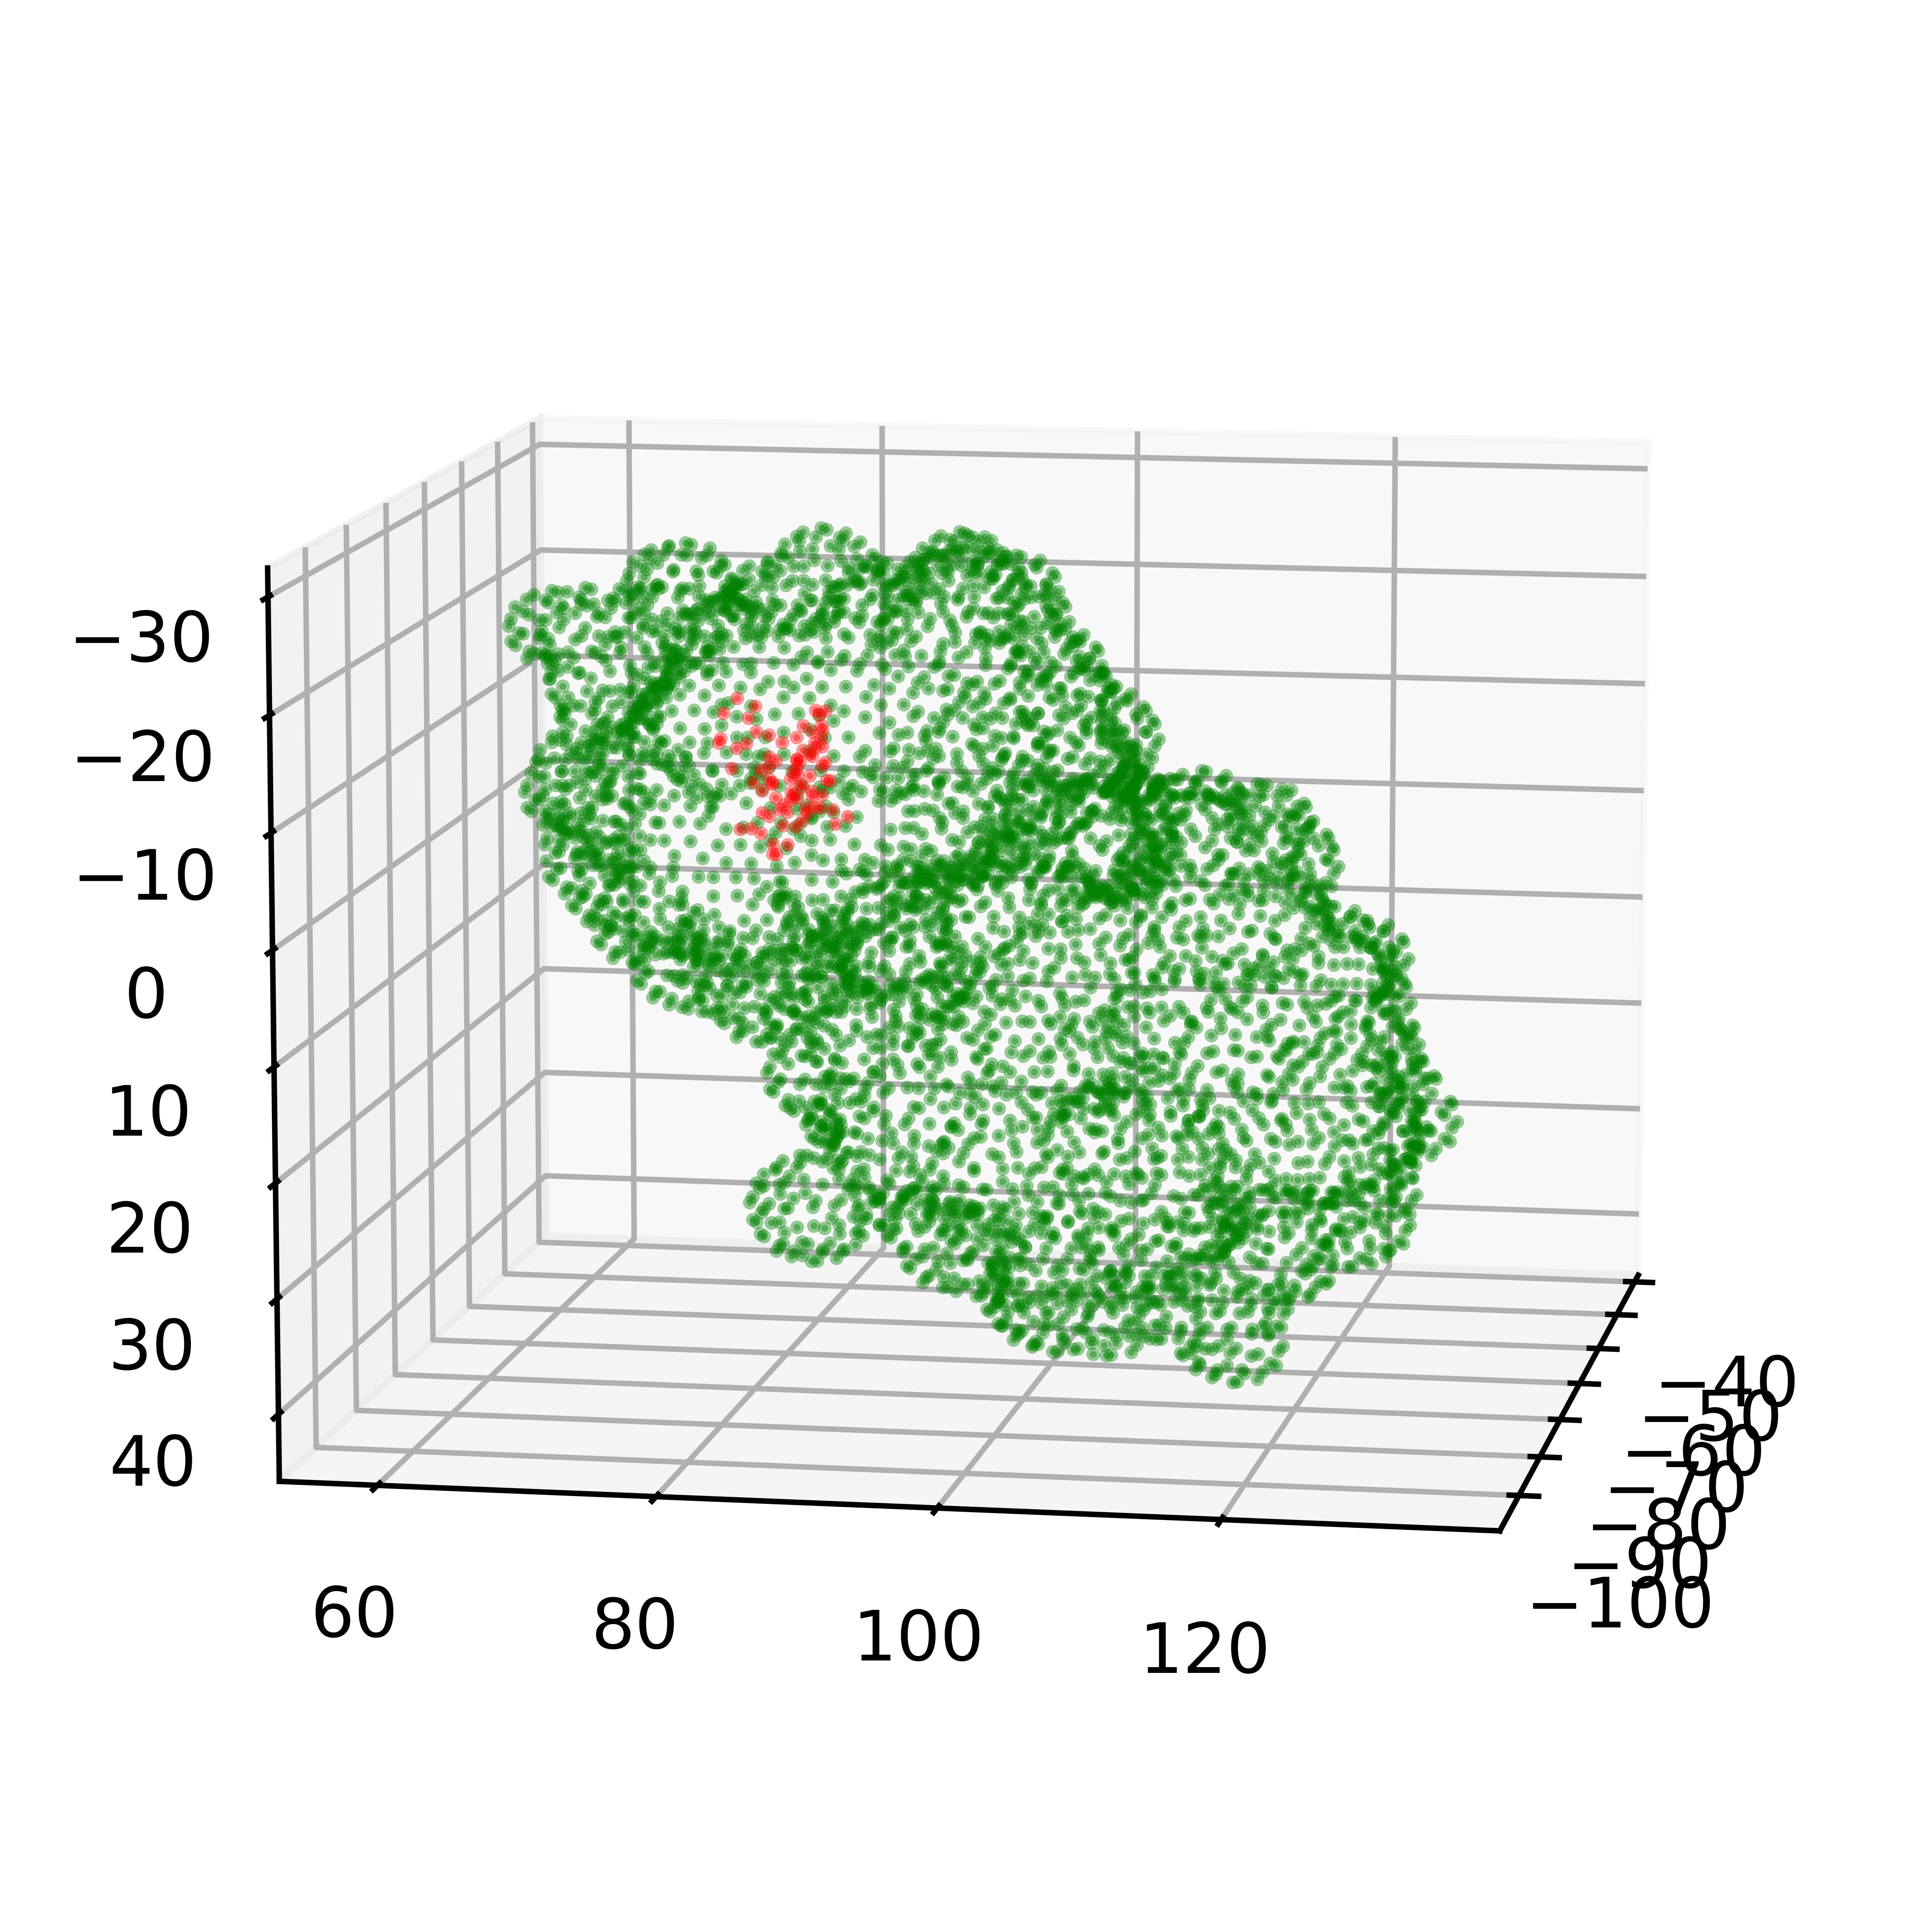
\includegraphics[width=1\linewidth]{point_cloud_class.png}
    \caption{SAS point cloud representing a protein with a highlighted ligand-binding site (in red). This point cloud is the input into the whole pipeline discussed in this work. Compare it to the P2Rank visualization in ~\ref{fig:p2rank_visualization} and feature visualization in 
    \label{fig:class_point_cloud}. This visualization was created by matplotlib.pyplot.scatter3D.}
\end{figure}

\begin{figure}
    \centering
    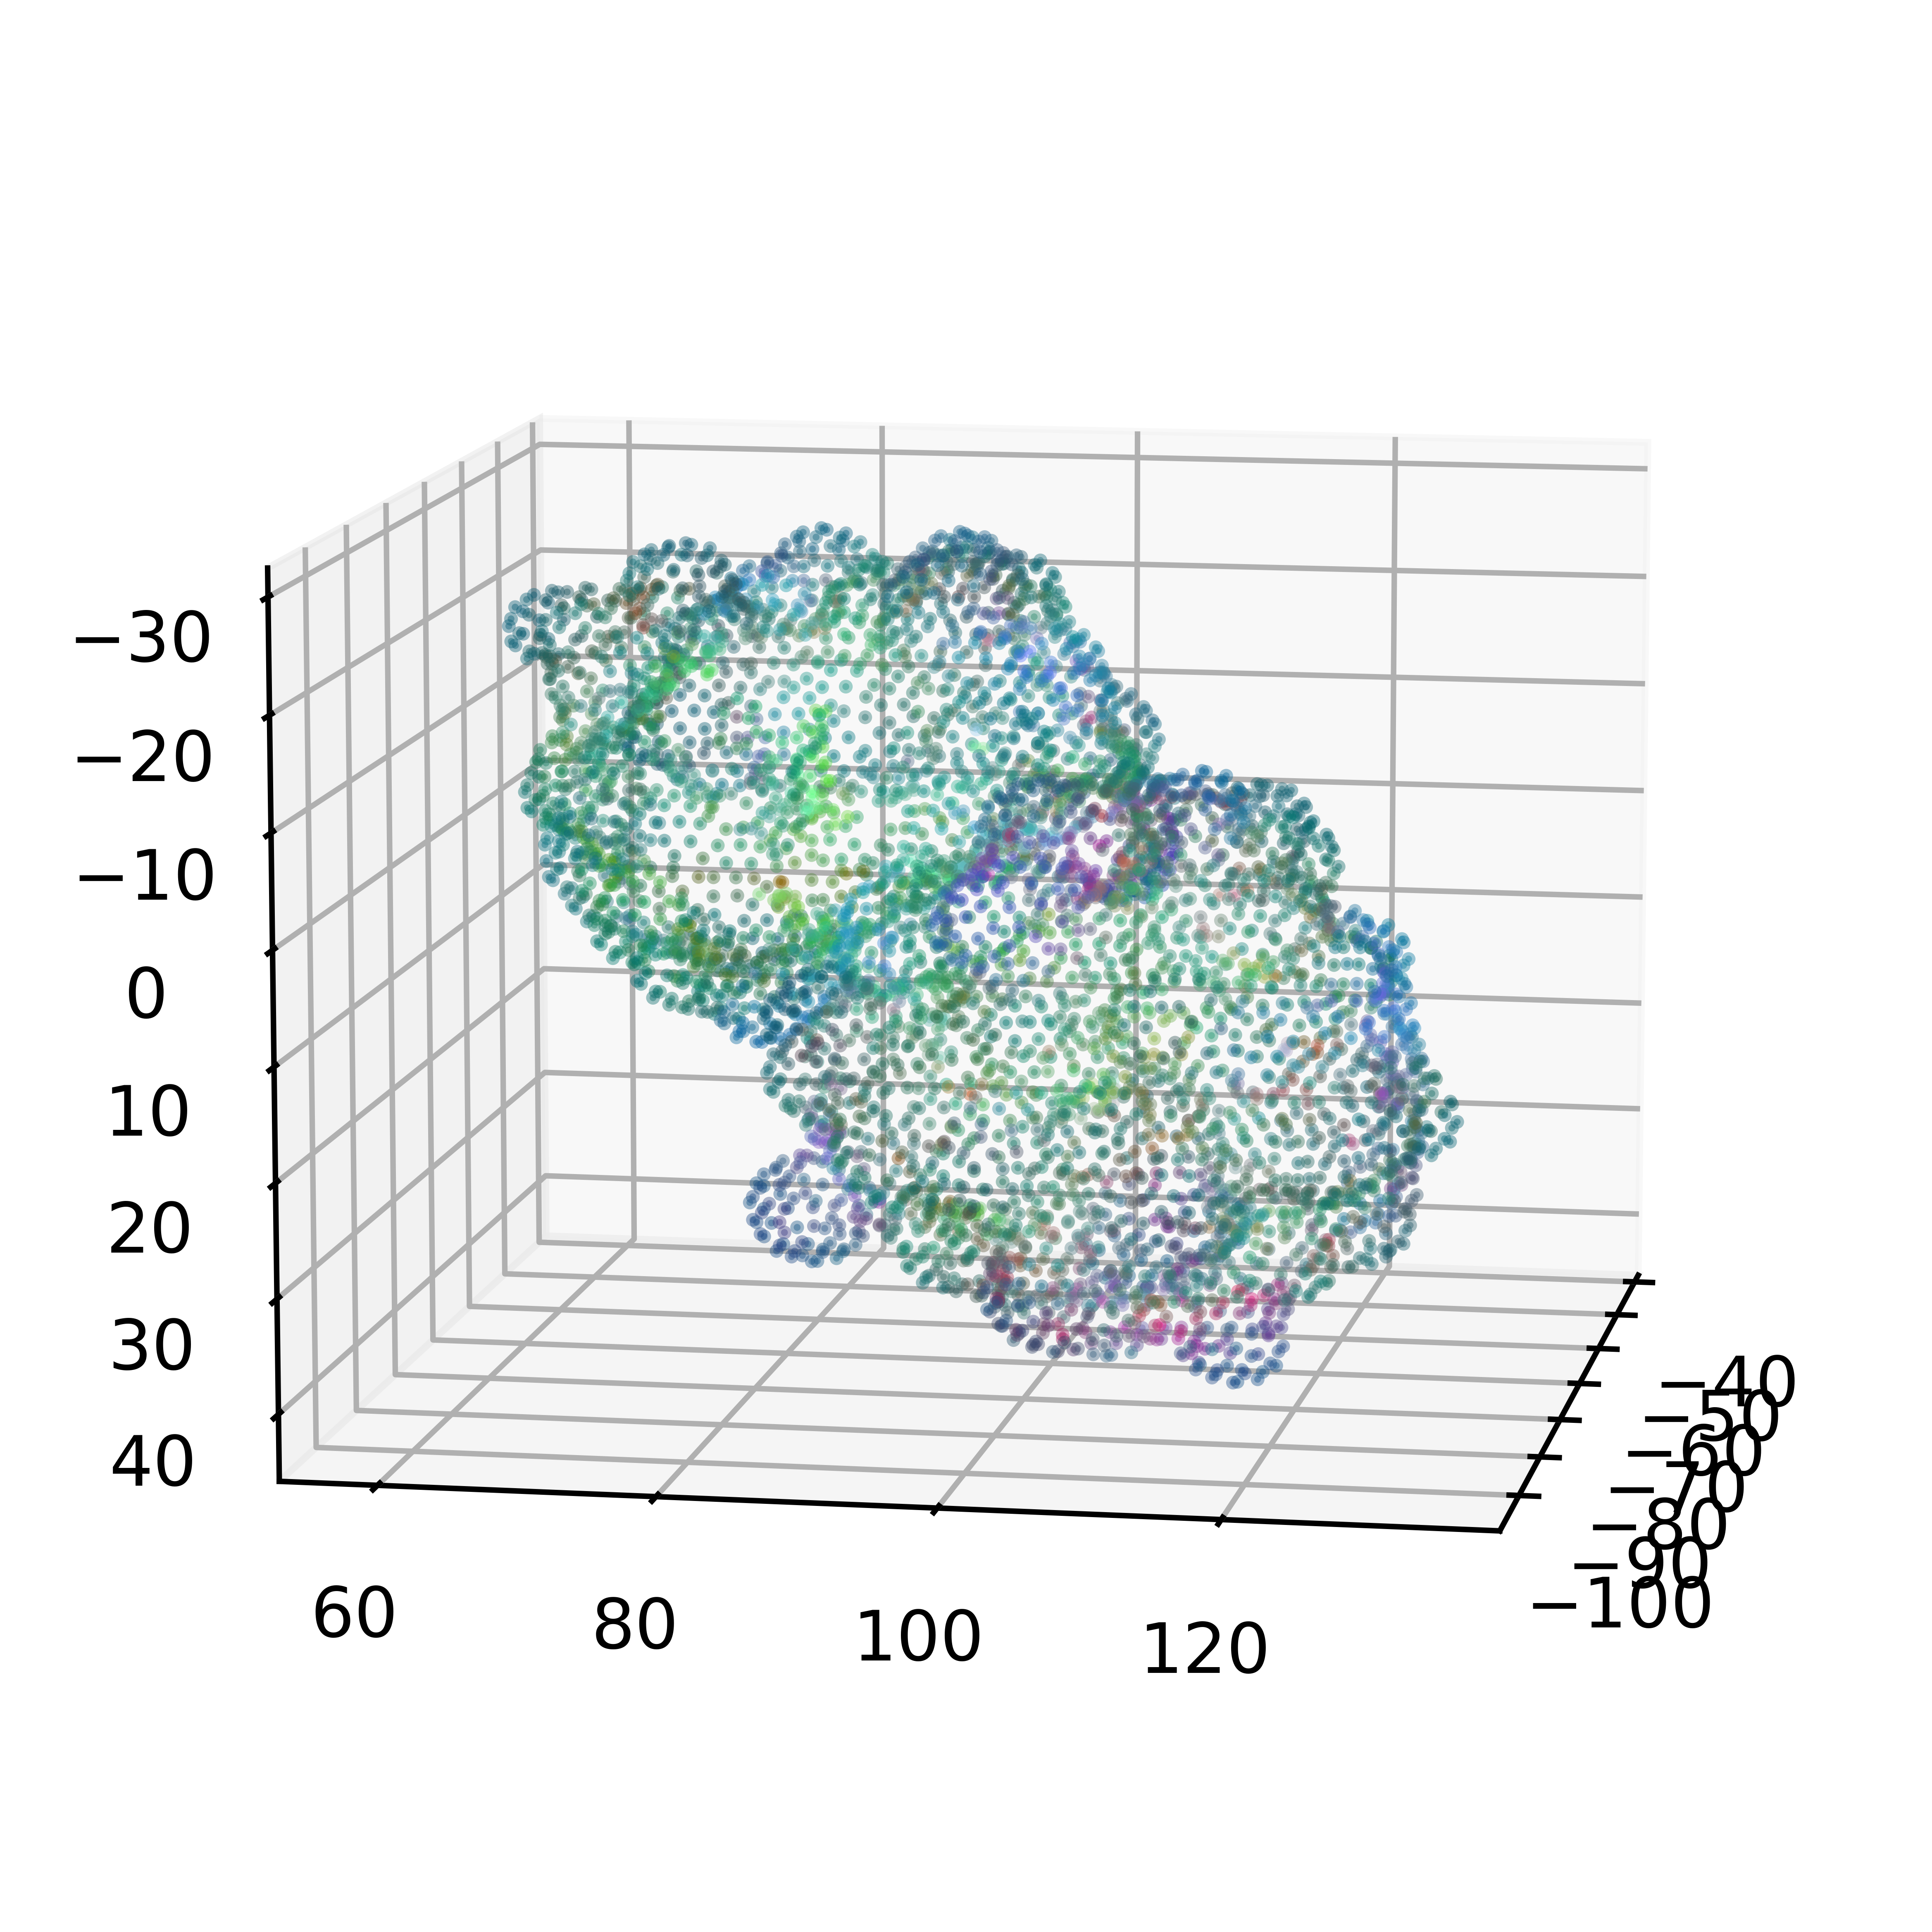
\includegraphics[width=1\linewidth]{point_cloud_pca.png}
    \caption{SAS point cloud showing the distribution of features across the surface. To achieve this visualization, locational and class-defining features were removed. Scikit-learn's PCA then reduced the remaining 35 dimensions to 3 dimensions. These were then plotted as red, green and blue channels using matplotlib.pyplot.scatter3D. It can be seen that there are no major feature outliers in the LBS area.}
    \label{fig:pca_point_cloud}
\end{figure}

In the implementation, these points are represented as tabular data, with three columns representing the X, Y, and Z axis, respectively. From this data, the point cloud can be recreated.

\subsection{Ligand-binding sites}

LBS represent protein parts, where a ligand (another chemically active substance) can bond to the protein. In datasets used in this work, the ligand can be any chemical substance passing some essential criteria. These limit the size (not too small, not too big) and chemical bond type (for example, ions are excluded, as these use a different mechanism of chemical bond).

Clusters of points represent LBS in our data. There is usually exactly one LBS per protein, but more can also exist. In some cases, no LBS is in the whole protein (but most of these proteins have been filtered out during the data preprocessing).

\subsection{Features}

As mentioned above, each point from the cloud has a feature vector attached. These features are fully described in the following section. The exact features are essential for result reproducibility, however, they are not crucial for understanding these experiments. 

These features represent chemical properties of the protein surface (such as hydrophobicity), surface shape (protrusion), or physical properties (XYZ coordinates). All of them represent a float value and are used as such - no binary or class features are used (atomic number could be seen as a class feature, but similarly sized atoms will have some similarities in their properties, so this feature is used as a numeric one as well).

\subsection{Exact datasets}

Two datasets were used in this work, taken from the original P2Rank paper. First of them is \textbf{CHEN11}, a dataset of 251 proteins harboring 476 ligands introduced in LBS prediction benchmarking study by \cite{chen11}. This dataset is used in the original paper as the training set and is used the same way in this work. A more detailed description is available in \cite{chen11}.

For model evaluation, the \textbf{COACH420} dataset is used. This dataset is shown in P2Rank as well. It is the test dataset from COACH(\cite{coach1}, \cite{coach2}), with all the proteins from the CHEN11 (and one other dataset from P2Rank) removed. 

\subsection{Surroundings extraction}
\label{Surroundings}

As described in the previous chapter, for the proposed algorithm to work, we need to have more features.

To achieve this, we run the following algorithm to extract the surroundings (some parts were simplified compared to the actual code by omitting performance improvements and ignoring some syntactical parts for the reasons of readability):

\begin{lstlisting}
def extract_surroundings(protein: pd.DataFrame, size: int, labels: pd.Series) -> np.array:
  surroundings_dataset = []
  for i in range(len(protein)):
    surroundings_datasetFor.append(
      protein.sort(key = lambda x: mahattan_distance(i, x)
        )[:size].flatten()
      )
  return surroundings_dataset, labels
\end{lstlisting}

Or, in natural language, for each point in the original protein surface, we take the $k$ nearest points to the original point. All features from these points are then concatenated, and labels are kept from the original data.

Having a larger context naturally improves the performance of any model. In \cite{P2RANK}, proposing this dataset, a larger context area is not considered in the models themselves but as a postprocessing step, where clusters of positively predicted points are used for LBS identification.
